%======================================================================
% PoznQMI-6.pdf
%======================================================================
\section{Částice ve 3D}
\strana{QM-C3-1}

\kw{Stavový prostor} \quad $\mathcal{H} = L^2(\mathbb{R}^3) = \mathcal{H}_1\otimes\mathcal{H}_1\otimes\mathcal{H}_1$ \\
\underline{ÚSKO:} \quad (úplné syst.\ komutujících oper.\ $=$ různé reprezentace)

\subsection*{1) \underline{Operátory polohy}: \ $\hat{\vec X} = (\hat x_1,\hat x_2,\hat x_3)$ \ \pozn{$=$ ÚSKO}}
$\to$ souřadnicová reprezentace: \quad $\braket{x_1,x_2,x_3}{\psi} \equiv \psi(x_1,x_2,x_3) \equiv \psi(\vec x)$
\[
  \braket{\psi}{\psi'} = \int\psi^*(\vec x)\,\psi'(\vec x)\,\dd^3x
\]

\subsection*{2) \underline{Operátor hybnosti (impulzu)} \ \dots\ $\hat{\vec P} = (\hat p_1,\hat p_2,\hat p_3)$ \ \pozn{$=$ ÚSKO}}
transformace $x\leftrightarrow p$:
\[
  \braket{\vec x}{\vec p} \equiv \braket{x_1x_2x_3}{p_1p_2p_3} = \vzorec{\frac{1}{\sqrt{(2\pi\hbar)^3}}\,e^{\frac{i}{\hbar}\vec p\cdot\vec x}}
\]
\hfill $\uparrow$ vl.\ fce odp.\ vl.\ č.\ $(p_1,p_2,p_3) = \vec p$

$\to$ v $x$-reprezentaci \quad $\vec p\,\psi(\vec x) = -i\hbar\vec\nabla\psi(\vec x)$

$\to$ normalizace k $\delta$: \quad $\braket{\vec p}{\vec p\,'} = \delta(\vec p - \vec p\,')$ \quad
$\big[= \delta(p_1 - p_1')\,\delta(p_2 - p_2')\,\delta(p_3 - p_3')\big]$

\pozn{ověření: $\displaystyle\int\dd^3\vec x\,\frac{1}{(2\pi\hbar)^3}e^{\frac{i}{\hbar}\vec x(\vec p\,' - \vec p)}
 = \frac{1}{(2\pi)^3}\int\frac{\dd x_1}{\hbar}e^{i\frac{x_1}{\hbar}(p_1'-p_1)}\int\frac{\dd x_2}{\hbar}e^{i\frac{x_2}{\hbar}(p_2'-p_2)}\int\frac{\dd x_3}{\hbar}e^{i\frac{x_3}{\hbar}(p_3'-p_3)}$} \\
\hspace*{3cm}\pozn{$\displaystyle = \frac{1}{(2\pi)^3}\,2\pi\delta(p_1'-p_1)\,2\pi\delta(p_2'-p_2)\,2\pi\delta(p_3'-p_3) = \delta(\vec p\,' - \vec p)$}

\subsection*{3) \underline{Energie a směr hybnosti} \ \pozn{$=$ ÚSKO}}
\dots\ volná částice \quad $\hat H_0 = \dfrac{p^2}{2m} = \dfrac{1}{2m}\sum_\alpha\hat p_\alpha\cdot\hat p_\alpha$; \quad $\vec n = \dfrac{\vec p}{p}$

platí \quad $[\hat p_\alpha,\hat p_\beta] = 0$ \quad $\to$ \quad $[\hat p_\alpha,\hat H_0] = 0$ \qquad $H_0 = f(p_\alpha)$; \ $\vec n = \vec g(p_\beta)$ \\
$\to$ vl.\ funkce $\ket{\vec p}$ jsou i vl.\ fcemi $\ket{E,\vec n}$ až na normování:
\[
  \braket{E,\vec n}{E',\vec n\,'} = \delta_2(\vec n - \vec n\,')\,\delta(E - E')
\]
\hspace*{3.5cm}\pozn{$\uparrow$ $\delta$-fce na 1 sféře} \quad \pozn{$\nwarrow$ $\delta$-fce na $\langle 0,\infty)$}

tj.\ \quad $\ket{E,\vec n} = N\ket{\vec p}$ \\
tj.\ \quad $\braket{E,\vec n}{E',\vec n\,'} = |N|^2\delta_3(\vec p - \vec p\,') = |N|^2\delta_1(p_1 - p_1')\,\delta_1(p_2 - p_2')\,\delta_1(p_3 - p_3')$ \\
\hspace*{4.5cm}\pozn{$\vec p = \vec p\,' + \Delta\vec p = \vec p\,' + (|p| - |p'|)\vec e_r + (\Delta n_\theta\vec e_\theta + \Delta n_\varphi\vec e_\varphi)\,p$}

\begin{minipage}{0.36\textwidth}
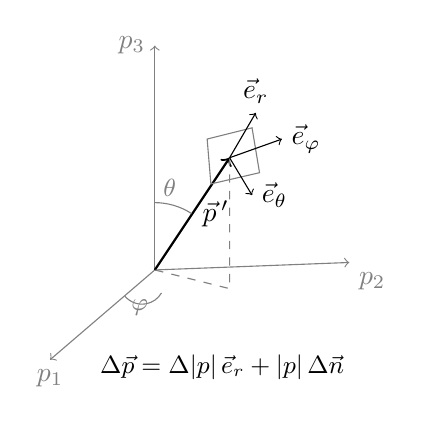
\begin{tikzpicture}[scale=0.95,gray]
  \coordinate (O) at (0,0);
  \draw[->] (O) -- (0,3) node[left] {$p_3$};
  \draw[->] (O) -- (2.6,0.1) node[below right] {$p_2$};
  \draw[->] (O) -- (-1.4,-1.2) node[below] {$p_1$};
  % vektor p'
  \draw[->,thick,black] (O) -- (1,1.5) node[midway,right] {$\vec p\,'$};
  \draw[thin] (0,0.9) arc (90:57:0.9); \node at (0.2,1.1) {\small$\theta$};
  \draw[thin] (-0.4,-0.35) arc (220:330:0.3); \node at (-0.2,-0.5) {\small$\varphi$};
  \draw[dashed,thin] (1,1.5) -- (1,-0.25) -- (O);
  % plošný element
  \draw[thin] (0.7,1.75) -- (1.3,1.9) -- (1.4,1.3) -- (0.75,1.15) -- cycle;
  \draw[->,black] (1,1.5) -- (1.35,2.1) node[above] {$\vec e_r$};
  \draw[->,black] (1,1.5) -- (1.7,1.75) node[right] {$\vec e_\varphi$};
  \draw[->,black] (1,1.5) -- (1.3,1.0) node[right] {$\vec e_\theta$};
  \node[black] at (0.9,-1.3) {\small$\Delta\vec p = \Delta|p|\,\vec e_r + |p|\,\Delta\vec n$};
\end{tikzpicture}
\end{minipage}
\begin{minipage}{0.62\textwidth}
\begin{align*}
  &= \frac{|N|^2}{p^2}\,\delta_2(\vec n - \vec n\,')\,\delta(|p| - |p'|) \\
  &\qquad \Big\lfloor\ p = \sqrt{2mE},\ \ \frac{\dd p}{\dd E} = \sqrt{\frac{m}{2E}} = \frac{m}{p} \\
  &= \frac{|N|^2}{p^2}\,\frac{p}{m}\,\delta_2(\vec n - \vec n\,')\,\delta(E - E')
  \quad\to\quad N = \sqrt{mp}
\end{align*}
\end{minipage}
\[
  \to\quad \vzorec{\ket{E\vec n} = \sqrt{mp}\,\ket{\vec p} = \sqrt{\frac{pm}{(2\pi\hbar)^3}}\;e^{\frac{i}{\hbar}\vec x\cdot\overbrace{\vec n\sqrt{2mE}}^{\vec p_{E,\vec n}}}}
\]

\pozn{Lamé $h_\theta, h_\varphi$ pro $r = 1$} \quad $\delta(\vec n - \vec n\,') = \delta(\theta - \theta')\,\delta\big(\sin\theta(\varphi - \varphi')\big)$

\underline{mimochodem:} tj.: \quad
$\displaystyle\int f(\vec n)\,\delta(\vec n - \vec n\,')\,\dd\Omega = f(\vec n\,')
 \overset{\text{na sféře}}{=} \int_0^\pi\!\!\int_0^{2\pi} f(\theta,\varphi)\,\delta(\theta - \theta')\frac{\delta(\varphi - \varphi')}{|\sin\theta|}\sin\theta\,\dd\varphi\,\dd\theta = f(\theta',\varphi')$

%----------------------------------------------------------------------
\strana{QM-C3-2}
\subsection*{4) \underline{Orbitální moment hybnosti} \ \pozn{do ÚSKO lze přibrat např.\ $E$ nebo $|\vec p|$}}
\[
  \hat L_\alpha = \varepsilon_{\alpha\beta\gamma}\underbrace{\hat Q_\beta}_{=\hat x}\hat P_\gamma
  \qquad\text{tj.}\quad \vec L = \vec X\times\vec P
\]
+ již dříve jsme ukázali: \quad $[L_\alpha,L_\beta] = i\hbar\,\varepsilon_{\alpha\beta\gamma}L_\gamma$ \quad \dots\ nelze hledat spol.\ vl.\ v.\ $L_1,L_2,L_3$

ale \quad $[L^2,L_1] = \underbrace{[L_1^2,L_1]}_{0} + [L_2^2,L_1] + [L_3^2,L_1]$
\[
  = -i\hbar\,(L_2L_3 + L_3L_2) + i\hbar\,(L_3L_2 + L_2L_3) = 0
\]
podobně \quad $[L^2,L_\alpha] = 0 \quad \forall\alpha = 1,2,3$

$\to$ \underline{standardní volby ÚSKO}: \quad $\{\hat A,\hat L^2,\underbrace{\hat L_z}_{=L_3}\}$ \quad kde $\hat A = |\hat p|$ nebo $\hat H_0$

\sout{operátory $L_\alpha, L^2$ v $x$ reprezentaci}

{\color{prbarva}\rule{\linewidth}{0.8pt}}
\subsection{Delší odbočka: Kvantová teorie momentu hybnosti}

obecně: sada operátorů splňující \quad $[J_\alpha,J_\beta] = i\hbar\,\varepsilon_{\alpha\beta\gamma}J_\gamma$ \\
\quad $\to$ reprezentace grupy rotací na $\mathcal{H}$; generátory $\uparrow$

\begin{itemize}
  \item def: \quad $J^2 \equiv J_\alpha J_\alpha$ \quad $\to$ \quad $[J^2,J_\alpha] = 0$
  \item $\Rightarrow$ $\exists$ sada vl.\ v.
  \[
    J^2\ket{\beta,m} = \hbar^2\beta\ket{\beta,m}, \qquad J_3\ket{\beta,m} = \hbar m\ket{\beta,m}
  \]
  \dots\ $\beta, m$ \dots\ bezrozměrné \quad \pozn{ještě může být degener.\ \dots\ další indexy $\alpha_1,\alpha_2$ \dots\ potlačíme}
  \item platí: \quad
  $\beta = \bra{\beta,m}\frac{J^2}{\hbar^2}\ket{\beta,m} = \bra{\beta,m}\big(\tfrac{J_1}{\hbar}\big)^2 + \big(\tfrac{J_2}{\hbar}\big)^2 + m^2\ket{\beta,m} \geq 0$ \\
  \hspace*{6cm} $\uparrow\quad\uparrow\ \geq 0$ \dots\ skal.\ součin $\to$ axiom $\braket{\psi}{\psi}\geq 0$ pro $\ket{\psi} = J_\alpha\ket{\beta m}$ \\
  tj.\ \quad $\beta \geq m^2 \geq 0$ \\
  \quad $\to$ spektrum $J_3$ je omezené
  \item \underline{posunovací operátory} a jejich vlastnosti:
  \[
    \text{def:}\ \ \boxed{\begin{aligned} J_+ &\equiv J_1 + iJ_2 \\ J_- &\equiv J_1 - iJ_2 \end{aligned}} = J_+^\dagger
    \quad\Rightarrow\quad
    \begin{aligned}
      {}[J_3,J_+] &= i\hbar J_2 - i(i\hbar)J_1 = \hbar J_+ &&(+)\\
      [J_3,J_-] &= -\hbar J_- &&(-)\\
      [J_+,J_-] &= i[J_2,J_1] - i[J_1,J_2] = 2\hbar J_3 &&(\pm)
    \end{aligned}
  \]
\end{itemize}

-- \underline{význam $J_+$:}
\[
  J_3\big(J_+\ket{\beta m}\big) = \big(J_+J_3 + \underbrace{[J_3,J_+]}_{(+)}\big)\ket{\beta m} = (\hbar m + \hbar)\,J_+\ket{\beta m}
\]
\quad $\to$ $J_+\ket{\beta m}$ je vl.\ v.\ $J_3$ odp.\ hodnotě $(m+1)$ nebo $0$-vý vektor

\quad {\color{prbarva}\underline{pozn:} $J_\pm\ket{\beta m}$ zůstávají vl.\ v.\ $J^2$ odpov.\ vl.\ č.\ $\hbar^2\beta$, neboť $[J^2,J_\pm] = 0$!}

-- \underline{význam $J_-$:}
\[
  J_3\big(J_-\ket{\beta m}\big) = \big(J_-J_3 + \underbrace{[J_3,J_-]}_{(-)}\big)\ket{\beta m} = \hbar(m-1)\,J_-\ket{\beta m}
\]
\quad $\to$ vl.\ v.\ $J_3$ pro $(m-1)$ nebo $0$

%----------------------------------------------------------------------
\strana{QM-C3-3}
\begin{itemize}
  \item \underline{maximální hodnota $m$}: $\overset{\text{def}}{\equiv} j$ \quad (existuje \dots\ spektrum $J_3$ omezené) \\
  musí \quad $\|J_+\ket{\beta,j}\|^2 = 0$ \\
  tj.\ \quad $\bra{\beta j}J_-J_+\ket{\beta j} = \bra{\beta j}\underbrace{J_1^2 + J_2^2 + i(J_1J_2 - J_2J_1)}\ket{\beta j} = \hbar^2(\beta - j^2 - j) = 0$ \\
  obecně: \quad $\hookrightarrow$ \quad $\boxed{J_-J_+ = J^2 - J_3^2 - \hbar J_3}\ \ (-+)$
  \quad $\Rightarrow$ \quad \underline{$\beta = j(j+1)$}

  podobně:
  \item \underline{minimální hodnota $m$}: $\equiv k$ \\
  \quad $J_-\ket{\beta k} = 0$ \\
  $\to$ $\bra{\beta k}J_+J_-\ket{\beta k} = \bra{\beta k}\underbrace{J_-J_+ + [J_+,J_-]}\ket{\beta k} = \hbar^2(\beta - k^2 + k) = 0$ \\
  \quad $\hookrightarrow$ \quad $\boxed{J_+J_- = J^2 - J_3^2 + \hbar J_3}\ \ (+-)$ \quad tj.\ $\beta = j(j+1) = k^2 - k$ \\
  \hspace*{5cm} $\Rightarrow$ \quad \underline{$k = -j$} \quad (nebo $(j+1) > j$, ale nemůže být min $>$ max)

  \item \underline{závěr:}
  \begin{veta}[Spektrum momentu hybnosti]
    spektrum $J_3$: ($\hbar\,\times$) \quad $m = -j, -j+1,\dots,j$ \\
    \quad přičemž rozdíl $j - k = 2j$ = celé číslo $\Rightarrow$ \quad $j = 0,\tfrac12,1,\tfrac32,2,\dots$ \\
    tj.\ pro $\forall j$ $\exists$ $2j+1$ vektorů s různým $m$

    \underline{změna značení:}
    \[
      \vzorec{\begin{aligned}
        J_3\ket{jm} &= \hbar m\ket{jm} \qquad\dots\ m = -j,\dots,j \\
        J^2\ket{jm} &= \hbar^2 j(j+1)\ket{jm}
      \end{aligned}} \qquad (*)
    \]
  \end{veta}
  která $j$ se realizují záleží na $\mathcal{H}$ a konkr.\ tvaru $\hat J_\alpha$
\end{itemize}
\rule{0.75\linewidth}{0.3pt}

\begin{priklad}[PŘ:]
\begin{itemize}[nosep]
  \item částice se spinem $\frac12$: \quad
        $\vec J = \vec S = \frac{\hbar}{2}\vec\sigma = \frac{\hbar}{2}\left(\begin{pmatrix}0&1\\1&0\end{pmatrix},\begin{pmatrix}0&-i\\ i&0\end{pmatrix},\begin{pmatrix}1&0\\0&-1\end{pmatrix}\right)$ \\
        \dots\ víme, že \quad $[\sigma_\alpha,\sigma_\beta] = 2i\,\varepsilon_{\alpha\beta\gamma}\sigma_\gamma$ \quad $\to$ \quad $[J_\alpha,J_\beta] = i\hbar\,\varepsilon_{\alpha\beta\gamma}J_\gamma$ \\
        \dots\ $\sigma_z$ má vl.\ č.\ $\pm 1$ $\Rightarrow$ $S_z$ vl.\ č.\ $\pm\hbar/2$ \quad \dots\ odpovídá $j = \frac12$
  \item za chvíli ukážeme, že $L_\alpha = \varepsilon_{\alpha\beta\gamma}Q_\beta P_\gamma$ odpovídá ($j =$) $l = 0,1,2,\dots$
\end{itemize}
\end{priklad}

\begin{itemize}
  \item \underline{normalizace:} \\
  \quad $J_+\ket{jm} = C\ket{j\,m+1}$ \quad \dots\ už víme $\bra{jm}J_-J_+\ket{jm} \overset{(-+)}{=} \hbar^2\big[j(j+1) - m(m+1)\big]$
  \[
    \to\quad \vzorec{J_+\ket{jm} = \hbar\sqrt{j(j+1) - m(m+1)}\,\ket{j\,m+1} = \hbar\sqrt{(j-m)(j+m+1)}\,\ket{j\,m+1}}
  \]
  podobně z $(+-)$:
  \[
    \vzorec{J_-\ket{jm} = \hbar\sqrt{j(j+1) - m(m-1)}\,\ket{j\,m-1} = \hbar\sqrt{(j+m)(j-m+1)}\,\ket{j\,m-1}}
  \]
  \dots\ podobně jako u LHO \dots\ obsahuje fázovou konvenci \\
  vektor o němž víme jen $(*)$ $\to$ $e^{i\alpha}\ket{jm}$! \quad \pozn{OBECNĚ}
\end{itemize}

%----------------------------------------------------------------------
\strana{QM-C3-4}
\begin{itemize}
  \item \underline{Maticová reprezentace $J_1,J_2,J_3$ ve vl.\ podpr.\ $J^2$} \\
  \pozn{souvisí s ireducibilními reprezent.\ grupy rotací \dots\ viz teor.\ grup} \\
  $\to$ $J^2, J_z$ se doplní na ÚSKO: $J^2, J_z, A$ \ $\to$ $\ket{\alpha,jm}$ \hfill $[A,J^2] = 0$, \ $[A,J_z] = 0$ \\
  \hspace*{4.3cm} $\hookrightarrow$ diagonální v $\circlearrowleft$ \hfill \pozn{předp.: $[A,J_\alpha] = 0\ \forall\alpha$}
  \begin{align*}
    \text{tj.}\quad \bra{\alpha,jm}J^2\ket{\alpha',j'm'} &= \hbar^2 j(j+1)\,\delta_{jj'}\delta_{mm'}\delta_{\alpha\alpha'} \\
    \bra{\alpha,jm}J_z\ket{\alpha',j'm'} &= \hbar m\,\delta_{jj'}\delta_{mm'}\delta_{\alpha\alpha'} \\
    \bra{\alpha,jm}J_1\ket{\alpha',j'm'} &= (J_1)^{(j)}_{mm'}\,\delta_{jj'}\delta_{\alpha\alpha'} \qquad\text{podob.\ } J_2
  \end{align*}
  $(J_1)_{mm'}$ lze najít explicitně: \quad $J_1 = \frac12(J_+ + J_-)$, \quad $J_2 = \dfrac{J_+ - J_-}{2i}$ \\
  + už víme \quad $\bra{\alpha,jm}J_+\ket{\alpha',j'm'} = \delta_{\alpha\alpha'}\delta_{jj'}\underbrace{\delta_{m\,m'+1}\,\hbar\sqrt{j'(j'+1) - m'(m'+1)}}_{(J_+)_{mm'}}$ \\
  \hspace*{4cm} $J_- = J_+^\dagger$
\end{itemize}

\textbf{ČÁSTICE SE SPINEM} $1/2, 1, 3/2,\dots$ atd.; pro celé $j$ $\to$ orb.\ moment

\pozn{TABULKA:}
\begin{center}
\renewcommand{\arraystretch}{1.3}
\begin{tabular}{c|c|c|c|c|c}
 & \fbox{$j=0$} & \fbox{$j=\frac12$} & \fbox{$j=1$} & \fbox{$j=\frac32$} & \\ \hline
$J_+ =$ & $(0)$ &
$\hbar\begin{pmatrix}0&1\\0&0\end{pmatrix}$ &
$\hbar\begin{pmatrix}0&\sqrt2&0\\0&0&\sqrt2\\0&0&0\end{pmatrix}$ &
$\hbar\begin{pmatrix}0&\sqrt3&0&0\\0&0&\sqrt4&0\\0&0&0&\sqrt3\\0&0&0&0\end{pmatrix}$ & $\cdots$ \\ \hline
$J_x =$ & &
$\frac{\hbar}{2}\begin{pmatrix}0&1\\1&0\end{pmatrix}$ &
$\frac{\hbar}{\sqrt2}\begin{pmatrix}0&1&0\\1&0&1\\0&1&0\end{pmatrix}$ &
$\frac{\hbar}{2}\begin{pmatrix}0&\sqrt3&0&0\\ \sqrt3&0&\sqrt4&0\\0&\sqrt4&0&\sqrt3\\0&0&\sqrt3&0\end{pmatrix}$ & $\cdots$ \\ \hline
$J_y =$ & &
$\frac{\hbar}{2}\begin{pmatrix}0&-i\\ i&0\end{pmatrix}$ &
$\frac{\hbar}{\sqrt2}\begin{pmatrix}0&-i&0\\ i&0&-i\\0&i&0\end{pmatrix}$ &
$\frac{\hbar}{2}\begin{pmatrix}0&-i\sqrt3&0&0\\ i\sqrt3&0&-i\sqrt4&0\\0&i\sqrt4&0&-i\sqrt3\\0&0&i\sqrt3&0\end{pmatrix}$ & $\cdots$
\end{tabular}
\end{center}
{\small (řádky/sloupce indexovány $m, m' = j, j-1, \dots, -j$; \ např.\ pro $j = \frac32$: $\frac32, \frac12, -\frac12, -\frac32$)}

{\color{teal}\rule{\linewidth}{0.8pt}}\\[-4pt]
\hfill{\color{teal}konec odbočky}

\underline{zpět orbitální moment hybnosti:} \\
\quad $L_\alpha$ splňují komut.\ relace generátorů rotací \\
\quad $\Rightarrow$ $\exists$ báze $\ket{\alpha,lm}$: \quad
$\begin{aligned}[t] L^2\ket{\alpha,lm} &= \hbar^2 l(l+1)\ket{\alpha,lm} \\ L_z\ket{\alpha,lm} &= \hbar m\ket{\alpha,lm}\end{aligned}$ \\
\quad kde $m = -l,\dots,l$, ale nevíme, jaká $l$ jsou dovolená \\
\quad ($\sigma(L^2)$ je podmnožinou $\{0,\frac12,1,\frac32,2,\dots\}$)

%----------------------------------------------------------------------
\strana{QM-C3-5}
\begin{itemize}
  \item \underline{operátor $\vec L$ v $x$-reprezentaci} \\
  samosdruženost: \quad $L_\alpha^\dagger = \varepsilon_{\alpha\beta\gamma}P_\gamma^\dagger Q_\beta^\dagger = \varepsilon_{\alpha\beta\gamma}Q_\beta P_\gamma = L_\alpha$ \\
  \hspace*{5cm} $\uparrow$ $Q^\dagger = Q$, $P^\dagger = P$; \ $[Q_\beta,P_\gamma] = 0$ pro $\gamma\neq\beta$
  \[
    \vec L = \vec Q\times(-i\hbar\vec\nabla_Q) \quad\dots\quad
    \begin{aligned}
      L_x &= -i\hbar\big(y\partial_z - z\partial_y\big), \qquad L_y = -i\hbar\big(z\partial_x - x\partial_z\big) \\
      L_z &= -i\hbar\big(x\partial_y - y\partial_x\big)
    \end{aligned}
  \]
\end{itemize}

\underline{pozn:} \underline{$p$-reprezentace:}
\[
  \vec L = (i\hbar\vec\nabla_p)\times\vec p = -i\hbar\,\vec p\times\vec\nabla_p
  \quad\dots\ \text{např.:}\ L_x = -i\hbar\Big(p_y\pdv{p_z} - p_z\pdv{p_y}\Big)
\]
\dots\ totožný tvar $\Rightarrow$ $\braket{\vec x}{lm}$; $\braket{\vec p}{lm}$ budou mít totožné funkční tvary (až na fázi) \\
\hspace*{2cm} (jen úhlová závislost)

\underline{vyjádření ve sférických souřadnicích:}

\begin{minipage}{0.32\textwidth}
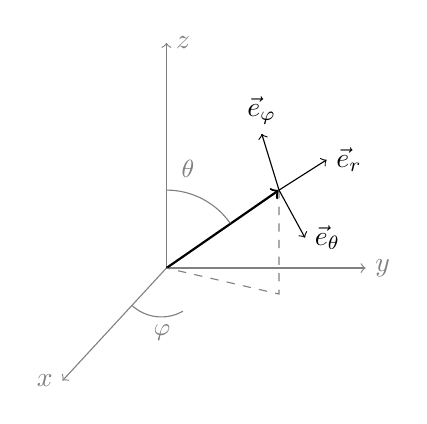
\begin{tikzpicture}[scale=1.1,gray]
  \coordinate (O) at (0,0);
  \draw[->] (O) -- (0,2.6) node[right] {$z$};
  \draw[->] (O) -- (2.3,0) node[right] {$y$};
  \draw[->] (O) -- (-1.2,-1.3) node[left] {$x$};
  \draw[->,thick,black] (O) -- (1.3,0.9);
  \draw[thin] (0,0.9) arc (90:35:0.9); \node at (0.25,1.15) {\small$\theta$};
  \draw[thin] (-0.4,-0.43) arc (227:300:0.5); \node at (-0.05,-0.75) {\small$\varphi$};
  \draw[dashed,thin] (1.3,0.9) -- (1.3,-0.3) -- (O);
  \draw[->,black] (1.3,0.9) -- (1.85,1.25) node[right] {$\vec e_r$};
  \draw[->,black] (1.3,0.9) -- (1.1,1.55) node[above] {$\vec e_\varphi$};
  \draw[->,black] (1.3,0.9) -- (1.6,0.35) node[right] {$\vec e_\theta$};
\end{tikzpicture}
\end{minipage}
\begin{minipage}{0.66\textwidth}
\begin{tabular}{l@{\qquad}ll}
$x = r\cos\varphi\sin\theta$ & Lamé: & $h_r = 1$ \\
$y = r\sin\varphi\sin\theta$ & & $h_\theta = r$ \qquad $h = \big\|\tfrac{\partial}{\partial\theta}(x,y,z)\big\|$ \\
$z = r\cos\theta$ & & $h_\varphi = r\sin\theta$
\end{tabular}
\end{minipage}
\[
  \boxed{\begin{aligned}
    \vec e_r &= \tfrac{\partial}{\partial r}(x,y,z) = \cos\varphi\sin\theta\,\vec e_x + \sin\varphi\sin\theta\,\vec e_y + \cos\theta\,\vec e_z \\
    h_\theta^{-1}\vec e_\theta &= \tfrac{\partial}{\partial\theta}(x,y,z) = \cos\varphi\cos\theta\,\vec e_x + \sin\varphi\cos\theta\,\vec e_y - \sin\theta\,\vec e_z \\
    h_\varphi^{-1}\vec e_\varphi &= \tfrac{\partial}{\partial\varphi}(x,y,z) = -\sin\varphi\,\vec e_x + \cos\varphi\,\vec e_y
  \end{aligned}}
\]
\underline{pozn:} \quad
$\begin{pmatrix}e_r\\ e_\theta\\ e_\varphi\end{pmatrix} = M\begin{pmatrix}e_x\\ e_y\\ e_z\end{pmatrix}$
\quad kde $M$ je OG matice: $M^{-1} = M^T$ \dots\ zpětná transf.

\underline{operátor $\vec L$:} \quad
$\boxed{\vec L = -i\hbar\,\vec Q\times\nabla = -i\hbar\,(r\vec e_r)\times\Big(\vec e_r\pdv{r} + \frac{\vec e_\theta}{h_\theta}\pdv{\theta} + \frac{\vec e_\varphi}{h_\varphi}\pdv{\varphi}\Big)}$ \\
\hspace*{5cm} přitom: \quad $\vec e_r\times\vec e_r = 0$, \quad $\vec e_r\times\vec e_\theta = \vec e_\varphi$, \quad $\vec e_r\times\vec e_\varphi = -\vec e_\theta$
\[
  \to\quad \vec L = -i\hbar\Big(\vec e_\varphi\pdv{\theta} - \frac{\vec e_\theta}{\sin\theta}\pdv{\varphi}\Big)
  = \begin{pmatrix}
      -i\hbar\big(-\sin\varphi\,\pdv{\theta} - \cos\varphi\,\frac{\cos\theta}{\sin\theta}\pdv{\varphi}\big) \\
      -i\hbar\big(\cos\varphi\,\pdv{\theta} - \sin\varphi\,\frac{\cos\theta}{\sin\theta}\pdv{\varphi}\big) \\
      -i\hbar\,\pdv{\varphi}
    \end{pmatrix}
  \begin{matrix} = L_x \\[8pt] = L_y \\[8pt] = L_z \end{matrix}
\]

\underline{pozn:} vyjádření $\vec L$ operátorů neobsahuje $r$! \dots\ působí jen na úhl.\ část. \\
\quad $\ket{lm}$ tvoří bázi v úhlových prom., tj.\ na 1-sféře \\
v ÚSKO $(L^2, L_z, A)$ \dots\ operátor $A$ dělá kvantování v $r$ \\
\hspace*{3cm} $A$ \dots\ komutuje s $\vec L$ $\to$ sfér.\ sym.\ \dots\ tj.\ skalár, \\
\hspace*{6cm} např.\ délka vektoru, stopa tenzoru
\[
  \vzorec{L_\pm = (L_x \pm iL_y) = \hbar e^{\pm i\varphi}\Big[\pm\pdv{\theta} + i\frac{\cos\theta}{\sin\theta}\pdv{\varphi}\Big]}
\]

%----------------------------------------------------------------------
\strana{QM-C3-6}
\begin{itemize}
  \item \underline{vyjádření $L^2$}
\end{itemize}
1) \quad $L^2 = -\hbar^2\Big[\vec e_\varphi\pdv{\theta} - \dfrac{\vec e_\theta}{\sin\theta}\pdv{\varphi}\Big]\Big[\vec e_\varphi\cdot\pdv{\theta} - \dfrac{\vec e_\theta}{\sin\theta}\cdot\pdv{\varphi}\Big]$

{\color{gray}
+ užití: \quad $\dfrac{\partial\vec e_\varphi}{\partial\theta} = 0$, \quad
$\dfrac{\partial\vec e_\varphi}{\partial\varphi} = -(\cos\varphi,\sin\varphi,0) = -\vec e_r\sin\theta - \vec e_\theta\cos\theta$ \\
\hspace*{1.4cm} $\dfrac{\partial\vec e_\theta}{\partial\theta} = -\vec e_r$, \quad $\dfrac{\partial\vec e_\theta}{\partial\varphi} = \cos\theta\cdot\vec e_\varphi$
\[
  \vzorec{L^2 = -\hbar^2\Big[\frac{\partial^2}{\partial\theta^2} + \frac{\cos\theta}{\sin\theta}\pdv{\theta} + \frac{1}{\sin^2\theta}\frac{\partial^2}{\partial\varphi^2}\Big]}
\]
\rule{0.6\linewidth}{0.3pt}

srovn.\ \dots\ $\Delta$ ve sfér.\ souř.
\begin{align*}
  \Delta &= \frac{1}{h_rh_\theta h_\varphi}\Big[\pdv{r}\frac{h_\theta h_\varphi}{h_r}\pdv{r} + \pdv{\theta}\frac{h_rh_\varphi}{h_\theta}\pdv{\theta} + \pdv{\varphi}\frac{h_rh_\theta}{h_\varphi}\pdv{\varphi}\Big] \\
  &= \underbrace{\frac{1}{r^2}\pdv{r}r^2\pdv{r}}_{\frac{\partial^2}{\partial r^2} + \frac2r\pdv{r}}
   + \frac{1}{r^2}\Big\{\underbrace{\frac{1}{\sin\theta}\pdv{\theta}\sin\theta\pdv{\theta}}_{\frac{\partial^2}{\partial\theta^2} + \frac{\cos\theta}{\sin\theta}\pdv{\theta}} + \frac{1}{\sin^2\theta}\frac{\partial^2}{\partial\varphi^2}\Big\}
   \quad \boxed{\{\ \} = -\frac{L^2}{\hbar^2r^2}}
\end{align*}
}

jiné odvození:
\[
  L^2 = -\hbar^2(\vec Q\times\vec\nabla)\cdot(\vec Q\times\vec\nabla) = -\hbar^2\big[(\vec Q\times\vec\nabla)\times\vec Q\big]\cdot\vec\nabla
\]
\[
  \overset{\text{BAC-CAB}}{=} -\hbar^2\big[(\vec Q\cdot\vec Q)\vec\nabla - \vec Q(\vec\nabla\cdot\vec Q)\big]\cdot\vec\nabla
  = -\hbar^2\Big\{r^2\Delta + r\pdv{r} - 3r\pdv{r} - \frac{\partial^2}{\partial r^2}\Big\}
\]
\hspace*{5.5cm} $\vec Q\cdot\nabla = r\pdv{r}$ \quad $\vec\nabla\vec Q = I$ \quad $\vec\nabla\cdot\vec Q = 3$
\[
  \text{tj.}\quad L^2 = -\hbar^2\Big(r^2\Delta - \frac{\partial^2}{\partial r^2} - 2r\pdv{r}\Big)
  \qquad \pozn{úhlová část $\Delta$-operátoru}
\]

\rule{\linewidth}{0.3pt}
\begin{itemize}
  \item \underline{vlastní podprostory $L^2, L_z$} \dots\ obecné pozn: \\
  \kw{homogenní polynomy stupně $l$} \dots\ $p_l(\lambda x,\lambda y,\lambda z) = \lambda^l p_l(x,y,z)$

  \pozn{PŘ: $x^2 + y^2 - \frac13z^2$ \dots\ $p_2(x,y,z)$; \quad $(x+iy)^3 = x^3 + 3ix^2y - 3xy^2 - iy^3$ \dots\ $p_3(x,y,z)$}

  platí:
  \begin{enumerate}[label=\arabic*)]
    \item $p_l(x,y,z) = r^l f(\theta,\varphi)$
    \item $L_\alpha\,p_l(x,y,z) = \tilde p_l(x,y,z)$ \quad $\swarrow$ opět homogenní st.\ $l$ \dots\ je vidět z $x$-repr.\ $L_\alpha$
    \item $\Delta\,p_l(x,y,z) = f(\theta,\varphi)\underbrace{\frac{1}{r^2}\pdv{r}r^2\pdv{r}r^l}_{l(l+1)r^{l-2}} - \frac{L^2}{\hbar^2}r^{l-2}f(\theta,\varphi)$ \\
    tj.\ pokud $\Delta p_l(x,y,z) = 0$ \quad $\Rightarrow$ \quad $L^2f(\theta,\varphi) = \hbar^2 l(l+1)f(\theta,\varphi)$
    \item pokud $\Delta p_l = 0$ \quad $\Rightarrow$ \quad $\Delta\tilde p_l = 0$, \quad kde $\tilde p_l = L_\alpha p_l$ \\
    \dots\ plyne z $[L^2,L_\alpha] = 0$ a vyjádření $\Delta$ pomocí $L^2$
  \end{enumerate}
\end{itemize}

%----------------------------------------------------------------------
\strana{QM-C3-7}
\underline{závěr:} $\ket{lm}$ lze hledat v prostoru polynomů \\
\hspace*{1.6cm} \dots\ homogenních stupně $l$ splňujících $\Delta p = 0$

-- počet homog.\ pol.\ stupně $l$: \\
\quad \pozn{$=$ počet koef.\ u $x^ay^bz^c$; $a+b+c = l$ $\to$ $(l+1) + l + \dots + 1 = \frac{(l+2)(l+1)}{2} = N(l)$}

počet $p_l$ splňujících $\Delta p_l = 0$: \\
\quad $\Delta$ mění stupeň $p_l$ o dva \dots\ $\Delta p = 0$ je $N(l-2)$ podmínek \\
\quad $\hookrightarrow$ $= N(l) - N(l-2) = \frac12\big[(l+2)(l+1) - l(l-1)\big] = 2l + 1$ \quad \dots\ konzistentní

\dots\ obvyklé značení \quad $f(\theta,\varphi) \equiv Y_{lm}(\theta,\varphi)$ \quad \dots \quad
{\color{gray}\fbox{$\begin{aligned} L^2Y_{lm} &= \hbar^2 l(l+1)Y_{lm} \\ L_zY_{lm} &= \hbar m\,Y_{lm}\end{aligned}$}}

$\to$ nalezení $Y_{lm}$: \quad \pozn{$-i\partial_\varphi Y = mY$} \\
{\color{gray}
\quad $\Rightarrow$ \quad $Y_{ll} = e^{im\varphi} = (\cos\varphi + i\sin\varphi)^m = \frac{1}{r^m}(x+iy)^m$ \quad $\leftarrow$ \\
\quad\quad $\to$ funguje jen pro $m = l$ \dots\ jinak netriv.\ $\theta$-část, ale ostatní pomocí $L_-$ \\
\quad nebo \quad $Y_{l,-m} = e^{-im\varphi} = (\cos\varphi - i\sin\varphi)^m = \frac{1}{r^m}(x-iy)^m$ \quad $\leftarrow$ \quad fáze?
}

\underline{tradiční způsob nalezení $Y_{lm}(\theta,\varphi)$} \dots\ separace proměnných
\[
  Y_{lm}(\theta,\varphi) = f(\theta)\,g(\varphi)
\]
\begin{itemize}
  \item $\to$ \quad $L_zg(\varphi) = -i\hbar\pdv{\varphi}g(\varphi) = \hbar m\,g(\varphi)$ \quad s period.\ podm.: $g(\varphi + 2\pi) = g(\varphi)$ \\
  $\to$ \quad $g(\varphi) = e^{im\varphi}$; \quad $m = 0,\pm1,\pm2,\dots$ \quad (+ z dřívějška víme $|m|\leq l$) \\
  \hspace*{6cm} $\to$ jen celočíselná $l$
\end{itemize}
+ dosazení $Y_{lm}(\theta,\varphi) = f(\theta)e^{im\varphi}$ do $L^2Y_{lm} = \hbar^2 l(l+1)Y_{lm}$:
\[
  -\Big[\frac{1}{\sin\theta}\pdv{\theta}\sin\theta\pdv{\theta} - \frac{m^2}{(\sin\theta)^2}\Big]f(\theta) = l(l+1)f(\theta)
\]
\hspace*{2cm} + substituce $z = \cos\theta$ \quad \dots\ $\dd z = -\sin\theta\,\dd\theta$ \hfill $\lambda\equiv l(l+1)$
\[
  \to\quad \Big\{\dv{z}\big[(1-z^2)\big]\dv{z} + \lambda - \frac{m^2}{1-z^2}\Big\}f(\theta) = 0
\]
\hspace*{6cm} hledáme řešení nesingulární v $\pm 1$

$\to$ \kw{přidružené Legendre funkce}:
\[
  \vzorec{Y_{lm}(\theta,\phi) = (-1)^m\sqrt{\frac{(2l+1)(l-m)!}{4\pi\,(l+m)!}}\;P_l^m(\cos\theta)\,e^{im\varphi}}
\]
\quad kde \quad $P_l^m(\xi) = \dfrac{1}{2^l l!}(1-\xi^2)^{m/2}\dfrac{\dd^{l+m}}{\dd\xi^{l+m}}(\xi^2 - 1)^l$

\begin{minipage}[t]{0.48\textwidth}
\underline{Relace ortogonality:}
\[ \int Y_{lm}^*(\vec n)\,Y_{l'm'}(\vec n)\,\dd\Omega_n = \delta_{ll'}\delta_{mm'} \]
\end{minipage}
\begin{minipage}[t]{0.5\textwidth}
\underline{Relace úplnosti:}
\[ \sum_{l=0}^\infty\sum_{m=-l}^{l} Y_{lm}(\vec n)\,Y_{lm}^*(\vec n\,') = \delta_2(\vec n - \vec n\,') \]
\pozn{$= \dfrac{\delta(\theta-\theta')\delta(\varphi-\varphi')}{|\sin\theta|} = \delta(\cos\theta - \cos\theta')\,\delta(\varphi - \varphi')$}
\end{minipage}

\pozn{rozebrat \dots\ $Y(\vec n) = Y(\theta,\varphi) = Y(\cos\theta,\varphi)$ \dots\ záměna diferenciálu; také v $\nearrow$}

%----------------------------------------------------------------------
\strana{QM-C3-8}
\subsubsection*{Detailnější odvození $Y_{lm}(\theta,\varphi)$}
\[
  0 = L_-Y_{l,-l}(\theta,\varphi) = \hbar e^{-i\varphi}\Big[-\pdv{\theta} + i\frac{\cos\theta}{\sin\theta}\pdv{\varphi}\Big]f(\theta)e^{-il\varphi}
  = \hbar e^{-i(l+1)\varphi}\Big[-\pdv{\theta} + l\frac{\cos\theta}{\sin\theta}\Big]f(\theta) = 0
\]
\quad tj.\ \quad $\dfrac{f'}{f} = l\dfrac{\cos\theta}{\sin\theta}$ \quad $\to$ \quad $f(\theta) = c_l(\sin\theta)^l$

$c_l$ z normalizace: \quad $\int\dd\varphi\int\sin\theta\,\dd\theta\,|c_l|^2\sin^{2l}\theta = 1$ \quad $\to$ \quad $c_l = \dfrac{1}{\sqrt{2\pi I}}$ \\
\quad kde \quad $I_l = \displaystyle\int_0^\pi\sin\theta\,\dd\theta\,\sin^{2l}\theta = \frac{2^{2l+1}(l!)^2}{(2l+1)!}$
\quad $\to$ \quad $c_l = \dfrac{\text{\sout{$(-1)^l$}}}{2^l l!}\sqrt{\dfrac{(2l+1)!}{4\pi}}$
\hfill \begin{tabular}[t]{l}\underline{fázová konvence} \\ $\to P_{l0}(\theta = 0) > 0$ \\ \dots\ $Y_{l0}(\theta,\varphi) > 0$\end{tabular}

\underline{trošku hraní s $L_+$:} \dots\ platí: \quad $\dfrac{\dd}{\dd(\cos\theta)} = -\dfrac{1}{\sin\theta}\cdot\dfrac{\dd}{\dd\theta}$
\begin{align*}
  \Rightarrow\quad \frac{\dd}{\dd\cos\theta}\big((\sin\theta)^{-m}f\big) &= -\frac{1}{\sin\theta}\big[(\sin\theta)^{-m}f' - m(\sin\theta)^{-m-1}\cos\theta\,f\big] \\
  &= -\sin^{-m-1}\theta\,\Big[f' - m\frac{\cos\theta}{\sin\theta}f\Big]
\end{align*}
\[
  \to\quad L_+fe^{im\varphi} = \hbar e^{i\varphi}\Big[\pdv{\theta} - m\frac{\cos\theta}{\sin\theta}\Big]f(\theta)e^{im\varphi}
  = -\hbar e^{i(m+1)\varphi}(\sin\theta)^{m+1}\frac{\dd}{\dd\cos\theta}\big[(\sin\theta)^{-m}f(\theta)\big]
\]
\[
  \Rightarrow\quad L_+^p fe^{im\varphi} = (-\hbar)^p e^{i(m+p)\varphi}(\sin\theta)^{m+p}\frac{\dd^p}{(\dd\cos\theta)^p}\big[(\sin\theta)^{-m}f\big]
\]
+ normování: \quad $L_+\ket{lm} = \hbar\sqrt{(l-m)(l+m+1)}\,\ket{l\,m+1}$
\[
  N\ket{lm} = (L_+)^{l+m}\ket{l,-l} = \hbar^{l+m}\sqrt{2l}\cdot\sqrt{2l-1}\cdots\sqrt{l-m+1}\cdot\sqrt1\cdot\sqrt2\cdots\sqrt{l+m}\;\ket{lm}
\]
\[
  \to\quad N = \frac{1}{\hbar^{l+m}}\sqrt{\frac{(l-m)!}{(l+m)!}\frac{1}{2l!}}
\]
vše dohromady:
\[
  \vzorec{Y_{lm}(\theta,\varphi) = \frac{(-1)^{l+m}}{2^l l!}\sqrt{\frac{2l+1}{4\pi}\frac{(l-m)!}{(l+m)!}}\;e^{im\varphi}(\sin\theta)^m\frac{\dd^{l+m}}{(\dd\cos\theta)^{l+m}}(\sin\theta)^{2l}}
\]
\quad + substituce \quad $\xi = \cos\theta$, \ $\sqrt{1-\xi^2} = \sin\theta$ \quad $\to$ vzorec na předch.\ str.

\underline{pozn:} $Y_{l0}(\theta)$ \dots\ Legendreův polynom (v prom.\ $\cos\theta$) \\
podrobněji: \quad
$Y_{l0}(\theta) = \dfrac{(-1)^l}{2^l l!}\sqrt{\dfrac{2l+1}{4\pi}}\;\underbrace{\dfrac{\dd^l}{\dd\xi^l}(1-\xi^2)^l\Big|_{\xi=\cos\theta}}_{\text{polynom st.\ } 2l-l}
 \equiv \sqrt{\dfrac{2l+1}{4\pi}}\,P_l(\cos\theta)$

relace ortogonality:
\[
  \delta_{ll'} = \int Y_{l0}(n)\,Y_{l'0}^*(n)\,\dd^2n = \int_0^{2\pi}\dd\varphi\int_0^\pi\underbrace{\sin\theta\,\dd\theta}_{\dd\xi}\sqrt{\frac{2l+1}{4\pi}}\sqrt{\frac{2l'+1}{4\pi}}\,P_l(\xi)P_{l'}(\xi)
\]
\[
  \to\quad \vzorec{\int_{-1}^{1}P_l(\xi)P_{l'}(\xi)\,\dd\xi = \frac{2}{2l+1}\delta_{ll'}}
  \qquad \begin{tabular}{l}\dots\ ortogonální polynomy \\ s vahou $w(\xi) = 1$ \\ na intervalu $\langle -1,1\rangle$ \\ $\to$ souvislost \dots\ Gauss\end{tabular}
\]

\underline{pozn:} symetrie: \quad $Y_{lm}(-\vec n) = Y_{lm}(\vec n)(-1)^l$ \\
\hspace*{3.25cm} $Y_{lm}^*(\vec n) = (-1)^m\,Y_{l,-m}(\vec n)$ \quad
\pozn{$\nearrow$ faktor $(-1)^m$ není vidět, dá se odv.\ podobně z $L_-$ operátoru (Cohen-Tannoudji)}

%----------------------------------------------------------------------
\strana{QM-C3-9}
\underline{pozn:} \kw{reálné harmoniky}: \quad
$\begin{aligned}[t]
  C_{lm} &= \tfrac{1}{\sqrt2}\big(Y_{lm} + Y_{lm}^*\big) \\
  S_{lm} &= \tfrac{1}{\sqrt2}\big(Y_{lm} - Y_{lm}^*\big) \quad\leftarrow \text{někdy se čistí faktorem } (-1)^{m+\dots}
\end{aligned}$ \hfill \fbox{$m\geq 0$} \\
\quad + $Y_{l0}$ beze změny

$\to$ $Y_{lm}^* \sim Y_{l,-m}$ \dots\ tj.\ jen unit.\ transf.\ v rámci $\pm m$ \\
$\to$ fázový faktor $e^{im\varphi}$ na 1-kouli $r = 1$: \\
\quad $\to$ je vždy doplněn faktorem $(\sin\theta)^m$: \quad $(r\sin\theta)^m e^{im\varphi} = (x + iy)^m$ \\
tj.\ \quad $C_{lm}\sim\cos m\varphi$, \quad $S_{lm}\sim\sin m\varphi$ \quad $\mathrm{Re}/\mathrm{Im}$ \dots\ $(x+iy)^m \pm (x-iy)^m$ \\
navíc $P_{lm}$ je vyjádř.\ $\sim\sin m\varphi\cdot\mathrm{poly}_{l-m}(\cos\theta)$ \dots\ homog.\ poly st.\ $m$

{\color{prbarva}\rule{\linewidth}{0.6pt}}\\[-4pt]
\hfill{\color{prbarva}konec odbočky}

\subsection*{4) \underline{ÚSKO obsahující $L^2, L_z$} \dots\ přidání $A$}
\dots\ většinou máme $[A,L_\alpha] = 0$ \quad $\to$ \quad $[A,L_\pm] = 0$ \\
\dots\ obecně \dots\ ve vl.\ podpr.\ $l,m$ diagonalizujeme $A$ $\to$ vl.\ č.\ $a_0,a_1,\dots,a_\alpha$ \\
\dots\ v principu $a$ závisí na $l,m$, ale \quad $AL_\pm\ket{a} = L_\pm A\ket{a}$ $\Rightarrow$ nezáv.\ na $m$
\[
  \to\quad
  \begin{aligned}
    L^2\ket{\alpha;lm} &= \hbar^2 l(l+1)\ket{lm,\alpha} && l = 0,1,2,\dots \\
    L_z\ket{lm,\alpha} &= \hbar m\ket{lm,\alpha} && m = -l,-l+1,\dots,l \\
    A\ket{lm,\alpha} &= a_\alpha^{(l)}\ket{lm,\alpha}
  \end{aligned}
\]
$\to$ spektrum $a$ závisí na konkr.\ volbě \dots\ kvantuje radiální prom.

\subsubsection*{4a) \underline{$A = H_0 \equiv p^2/2m$} -- řešení v $p$-reprezentaci}
$\to$ ihned \quad $\braket{\vec p}{Elm} = N\,\delta(E_p - E)\,Y_{lm}(\hat p)$ \qquad $\hat p \equiv \dfrac{\vec p}{|p|}$

normování: \quad $\braket{Elm}{E'l'm'} = \displaystyle\int\dd^3p\,|N|^2\delta\Big(E - \frac{p^2}{2m}\Big)\delta\Big(E' - \frac{p^2}{2m}\Big)Y_{lm}^*(\hat p)Y_{l'm'}(\hat p)$
\begin{align*}
  \hspace*{3cm} &= \delta_{ll'}\delta_{mm'}|N|^2\int p^2\,\dd p\,\frac{\delta(p - p_E)}{p/m}\,\delta\Big(E' - \frac{p^2}{2m}\Big) \\
  &= pm\,|N|^2\,\delta_{ll'}\delta_{mm'}\,\delta(E - E')
\end{align*}
\quad $N = \dfrac{1}{\sqrt{pm}}$ \pozn{$= (2Em^3)^{-1/4}$} \quad $\nwarrow$

\underline{závěr:} \quad $\vzorec{\braket{\vec p}{Elm} = \frac{1}{\sqrt{pm}}\,\delta\Big(E - \frac{p^2}{2m}\Big)\,Y_{lm}(\hat p)}$

\subsubsection*{4b) \underline{$A = H_0 \equiv p^2/2m$} -- řešení v $x$-reprezentaci}
$\to$ v principu Fourier.-transformace předchozího, ale def.\ spec.\ fce
\[
  \psi_{Elm}(\vec Q) = \int\dd^3p\,\braket{\vec x}{\vec p}\braket{\vec p}{Elm}
  \quad\dots\ \text{dá se odvodit z rozkladu:}
\]
\[
  \vzorec{e^{i\vec k\cdot\vec Q} = 4\pi\sum_l\sum_m i^l\,j_l(kr)\,Y_{lm}^*(\hat k)\,Y_{lm}(\hat Q)}
  \qquad \vec k \equiv \frac{\vec p}{\hbar}
\]
následující lze chápat jako odvození $\uparrow$ a definice $j_l(kr)$

%----------------------------------------------------------------------
\strana{QM-C3-10}
hledáme \quad $\psi_{klm}(\vec Q) \equiv \braket{\vec Q}{klm} = R_{kl}(r)\,Y_{lm}(\theta,\varphi)$ \\
\quad kde \quad $E = \dfrac{p^2}{2m}$, \quad $k = \dfrac{p}{\hbar} = \dfrac{\sqrt{2mE}}{\hbar}$ \quad \dots\ $H_0\ket{klm} = E\ket{klm}$

normování a skal.\ součin: \quad $\braket{klm}{k'l'm'} = \delta_{ll'}\delta_{mm'}\int\dd r\,r^2R_{k'l}^*R_{kl}$ \\
$\to$ je výhodné zavést \dots\ $\chi_{kl} \equiv r\,R_{kl}(r)$ \dots\ radiální skal.\ souč.: $\braket{\chi}{\chi'} = \int\chi^*\chi'\,\dd r$
\[
  \to\quad \psi_{klm}(\vec Q) = \frac{1}{r}\,\chi_{kl}(r)\,Y_{lm}(\theta,\varphi)
\]
\[
  H_0\psi_{klm}(\vec Q) = -\frac{\hbar^2}{2m}\Delta\psi_{klm} = -\frac{\hbar^2}{2m}\frac{1}{r^2}\Big[\pdv{r}r^2\pdv{r} - l(l+1)\Big]\psi = E\psi
\]
\[
  \to\quad \underbrace{R_{kl}''(r) + \frac2r R_{kl}'}_{\pozn{$\frac1r(rR)'' = \frac1r(R + rR')' = \frac1r(2R' + rR'')$}}
  + \Big[k^2 - \frac{l(l+1)}{r^2}\Big]R_{kl} = 0
\]
\hspace*{7cm} $\uparrow$ centrifugální člen (jako v klas.\ fyzice) \quad $\dfrac{L^2}{2mr^2}$
\[
  \to\quad \vzorec{\chi''(r) + \Big[k^2 - \frac{l(l+1)}{r^2}\Big]\chi(r) = 0}
  \quad\swarrow\ \text{jako 1D (SR) s } V_l(r) = \frac{\hbar^2 l(l+1)}{2mr^2}
\]

\underline{řešení pro $l = 0$:} \quad $\chi(r) = A\sin kr + B\cos(kr)$

\underline{okrajové podmínky:} \dots\ spojitost $\psi$ a $\psi'$ ($\nabla\psi$) v počátku \\
\hspace*{3.5cm} tj.\ $R(r = 0) = 0$ pro $l > 0$; \ $\chi_l(0) = 0$ $\forall l$

$\to$ bezrozm.\ jednotky: \quad $z = kr$ \quad $\to$ \quad $R(r) = j_l(kr) = j_l(z)$ \\
tj.\ \quad $\Big[\dfrac{\dd^2}{\dd z^2} + \dfrac2z\dfrac{\dd}{\dd z} + 1 - \dfrac{l(l+1)}{z^2}\Big]j_l(z) = 0$ \quad \dots\ univerz.\ rovnice nezáv.\ na $E$

\sout{nalezení asympt.\ chování \dots\ $j_l(z) = z^{l+1}$} \quad + def.\ $\hat j_l(z) = z\,j_l(z)$
\[
  \to\quad \hat j''(z) + \Big[1 - \frac{l(l+1)}{z^2}\Big]\hat j(z) = 0 \qquad\dots\ \text{asymptotika } \hat j \approx z^\alpha,\ z\to 0
\]
\quad \dots\ $\alpha(\alpha-1)z^{\alpha-2} - l(l+1)z^{\alpha-2} = 0$ \quad $\to$ \quad $\alpha = l+1$ \quad
{\color{gray}\fbox{\sout{$\alpha = -l$}} $\to$ nevyhovuje poč.\ podm.}

vytažení asymptotiky: \quad
$\begin{aligned}[t]
  \hat j(z) &= z^{l+1}\varphi(z) \\
  \hat j'(z) &= z^{l+1}\Big(\varphi' + \frac{l+1}{z}\varphi\Big) \\
  \hat j''(z) &= z^{l+1}\Big(\varphi'' + \frac2z(l+1)\varphi' + \frac{l(l+1)}{z^2}\varphi\Big)
\end{aligned}$

%----------------------------------------------------------------------
\strana{QM-C3-11a}
{\small\hfill (verze a)}
\[
  \to\quad \varphi'' + \frac2r(l+1)\varphi' + \varphi = 0
\]
\hspace*{5cm} \dots\ řešení $l = 0$: \quad $\varphi_0(z) = \dfrac{\sin z}{z}$ \quad (z rovn.\ pro $\hat j$)

+ \underline{pozorujte:} funkce $\psi = \dfrac{\varphi'}{r}$ splňuje: \quad $\psi'' + \dfrac{2(l+2)}{r}\psi' + \psi = 0$ \\
$\Rightarrow$ \quad $\varphi_{l+1}(z) = \psi(z) = \dfrac1z\dfrac{\dd}{\dd z}\varphi_l(z)$
\quad \dots\ přitom: $R_{kl}(r) = j(kr) = \dfrac{\hat j(kr)}{kr} = (kr)^l\varphi(kr)$

tj.\ \quad $R_{kl}(r) = C\,j(kr)$, \quad kde:
\[
  \vzorec{j_l(z) \equiv (-1)^l z^l\Big(\frac1z\frac{\dd}{\dd z}\Big)^l\frac{\sin z}{z}}
\]
\quad druhé lin.\ nez.\ řešení: \quad
$n_l(z) \equiv (-1)^{l+1}z^l\Big(\dfrac1z\dfrac{\dd}{\dd z}\Big)^l\dfrac{\cos z}{z}$

$\to$ \kw{sférické cylindrické funkce} \dots\ Besselova a Neumannova

\underline{asymptotické chování:} \quad $z\to 0$ \quad
$j_l(z) = \dfrac{z^l}{(2l+1)!!}$, \quad $n_l(z) = \dfrac{(2l+1)!!}{z^{l+1}}$ \quad \pozn{DK nebude}

$z\to\infty$ \quad \dots\ jen nejvyšší mocnina $z$: derivujeme jen $\sin/\cos$: \\
\quad přičemž \quad $\dfrac{\dd}{\dd z}\sin(z + \delta) = \sin\big(z - \tfrac{\pi}{2} + \delta\big)$ \quad $\to$
\[
  j_l(z) \xrightarrow{\ z\to\infty\ } \frac1z\sin\Big(z - \frac{\pi}{2}l\Big)
  \qquad n_l(z) = -\frac1z\cos\Big(z - \frac{\pi}{2}l\Big)
\]

\underline{Normování:} \quad platí \quad $\displaystyle\int_0^\infty j_l(kr)\,j_l(k'r)\,r^2\dd r = \frac{\pi}{2k^2}\delta(k - k')$

\underline{Důkaz:} z toho, že $H_0$ je samosdružený víme, že $\int j(kr)j(k'r)\sim\delta$ \\
\quad $\to$ zajímá nás jen singulární ($\delta$-chování) \\
posun o kvadraticky integ.\ fci neovlivní: \quad $\int(j_l - f)(j_l - f)\sim$ regulární $F(k,k') + \delta$

\dots\ stačí asymptotika:
\begin{align*}
  \int_0^\infty\sin(kr+\delta)\sin(k'r+\delta)\frac{1}{kk'}\,\dd r
  &= \frac{1}{kk'}\Big(-\frac14\Big)\int_0^\infty\underbrace{(e^{iA} - e^{-iA})(e^{iA'} - e^{-iA'})}_{e^{i(A+A')} + e^{-i(A+A')} - e^{i(A-A')} - e^{-i(A-A')}}\dd r \\
  &\hspace*{4cm}\hookrightarrow\ \sim\delta(k + k')\ \dots\ \text{nepřisp., } k,k' > 0 \\
  &= \frac{1}{2kk'}\int_{-\infty}^\infty\cos(k-k')r\,\dd r = \frac{1}{4kk'}\int_{-\infty}^\infty e^{i(k-k')r}\,\dd r \\
  &= \frac{2\pi}{4kk'}\,\delta(k - k')
  \quad\to\quad \text{\underline{normalizované}:}\ \vzorec{R_{kl}(r) = \sqrt{\frac{2}{\pi}}\,k\,j_l(kr)}
\end{align*}
\hfill ($\leftarrow\ \delta(k - k')$)

%----------------------------------------------------------------------
\strana{QM-C3-11b}
\subsubsection*{Algebraické řešení dle Cohena-Tannoudji {\normalfont\small(verze b)}}
\dots\ ukázali jsme: $\forall$ vektor: \quad $[L_\alpha,P_\beta] = i\hbar\,\varepsilon_{\alpha\beta\gamma}P_\gamma$
\begin{enumerate}[label=\arabic*)]
  \item[$\Rightarrow$ 1)] $[L_z,P_+] = [L_z,P_x] + i[L_z,P_y] = \hbar(iP_y + P_x) = \hbar P_+$ \\
        \hspace*{1.6cm} $\hookrightarrow$ def.\ \fbox{$P_+ = P_x + iP_y$}
  \item[2)] $[L_+,P_z] = [L_x,P_z] + i[L_y,P_z] = \hbar(-iP_y - P_x) = -\hbar P_+$
  \item[3)] $[L^2,P_+] = [L_y^2 + L_z^2,P_x] + i[L_x^2 + L_z^2,P_y] = \hbar\big[i(-L_yP_z - P_zL_y + L_zP_y + P_yL_z)$ \\
        \hspace*{7.4cm} $- L_xP_z - P_zL_x + L_zP_x + P_xL_z\big]$ \\
        $= \hbar\{L_zP_+ + P_+L_z - P_zL_+ - L_+P_z\} = 2\hbar(P_+L_z - P_zL_+) + \hbar\big(\underbrace{[L_z,P_+]}_{\hbar P_+} - \underbrace{[L_+,P_z]}_{-\hbar P_+}\big)$ \\
        $= 2\hbar(P_+L_z - P_zL_+) + 2\hbar^2P_+$
\end{enumerate}

\begin{veta}[Lemma]
\[ P_+\ket{klm}\Big|_{m=l} \sim \ket{k\,l{+}1,l{+}1} \]
\end{veta}
\underline{DK:}
\begin{itemize}[nosep]
  \item $[P_\alpha,H_0]$ $\Rightarrow$ $P_+\ket{klm}$ je vl.\ v.\ $H_0$ s vl.\ č.\ $E = \dfrac{\hbar^2k^2}{2m}$
  \item viz 2) \ $[L_z,P_+]$ $\Rightarrow$ $L_zP_+\ket{klm} = P_+L_z\ket{klm} + [L_z,P_+]\ket{klm} = \hbar(m+1)P_+\ket{klm}$
  \item 3) $\Rightarrow$ $L^2P_+\ket{klm}\big|_{m=l} = P_+L^2\ket{klm} + [L^2,P_+]\ket{kll} = \big[\hbar^2 l(l+1) + 2\hbar^2l - 0 + 2\hbar^2\big]P_+\ket{kll}$ \\
        \hspace*{3.4cm} $= \hbar^2(l+1)(l+2)\,P_+\ket{kll}$ \quad \dots\ + jednoznačnost
\end{itemize}
4) \quad $[P_+,x + iy] = [P_x,x] + (i)^2[P_y,y] = -i\hbar + i\hbar = 0$

\underline{Postup:}
\begin{center}
\begin{tikzpicture}[>=Stealth, node distance=1.8cm]
  \node (a) at (0,0) {$\ket{k00}$};
  \node (b) at (2.4,0) {$\ket{k11}$};
  \node (c) at (4.8,0) {$\ket{k22}$};
  \node (d) at (7,0) {$\dots$};
  \draw[->] (a) -- node[above] {$P_+$} (b);
  \draw[->] (b) -- node[above] {$P_+$} (c);
  \draw[->] (c) -- node[above] {$P_+$} (d);
  \node (b1) at (2.4,-1.2) {$\ket{k1m}$};
  \node (c1) at (4.8,-1.2) {$\ket{k2m}$};
  \node (d1) at (7,-1.2) {$\dots$};
  \draw[->] (b) -- node[right] {$L_-$} (b1);
  \draw[->] (c) -- node[right] {$L_-$} (c1);
  \draw[gray,double,->] (a) -- (0,-1.9);
  \draw[gray] (5.8,-0.6) -- (8.8,-0.6) -- (8.8,-2.1) -- (7,-2.1);
  \node[gray,right] at (8.9,-1.2) {\small$L_-$ působí jen na $\theta,\varphi$};
\end{tikzpicture}
\end{center}
přitom \quad $\braket{\vec Q}{klm} = N\,j_l(kr)\,Y_{lm}(\theta,\varphi)$ \\
$\to$ jak působí $P_+$? \quad \dots \quad $Y_{ll}(\theta,\varphi) = A(\sin\theta)^le^{il\varphi} = A\Big(\dfrac{x+iy}{r}\Big)^l$
\[
  P_+\frac{\sin kr}{kr}\ \dots\ -i\hbar(\partial_x + i\partial_y)f(r) \sim \underbrace{\Big(\pdv{r}{x} + i\pdv{r}{y}\Big)}_{\frac{x+iy}{r}}\pdv{f}{r}
  \sim \underbrace{(x+iy)}_{\sim\,Y_{11}(\theta,\varphi)}\frac1r\pdv{f}{r}
\]
indukce: \quad
$P_+(x+iy)^l\underbrace{\Big(\frac1r\pdv{r}\Big)^lf(r)}_{g(r)} = (x+iy)^lP_+g(r) \sim (x+iy)^{l+1}\frac1r\pdv{r}g(r)$ \\
\hspace*{8cm} $= (x+iy)^{l+1}\Big(\dfrac1r\pdv{r}\Big)^{l+1}f(r)$
\[
  \Rightarrow\ (\text{def})\quad j_l(z) \equiv (-1)^lz^l\Big(\frac1z\frac{\dd}{\dd z}\Big)^l\frac{\sin z}{z} \qquad\dots\ z = kr
\]
druhé LNZ řešení \quad $n_l(z) \equiv (-1)^{l+1}z^l\Big(\dfrac1z\dfrac{\dd}{\dd z}\Big)^l\dfrac{\cos z}{z}$

%----------------------------------------------------------------------
\strana{QM-C3-12}
\underline{chování pro malé $z$:} \\
\quad Taylorova řada pro $\sin z/\cos z$ \quad $\to$ \quad
$j_l(z) \underset{z\to0}{\approx} \dfrac{z^l}{(2l+1)!!}$, \qquad $n_l(z) \approx \dfrac{(2l+1)!!}{z^{l+1}}$

\underline{Asymptotické chování pro velké $z$:} \\
\dots\ největší mocnina $z$ \dots\ derivujeme jen $\sin/\cos$:
\[
  \frac{\dd}{\dd z}\sin(z+\delta) = \sin\Big(z - \frac{\pi}{2} + \delta\Big)
  \ \underset{z\to\infty}{\to}\
  \vzorec{j_l(z) \simeq \frac1z\sin\Big(z - \frac{\pi}{2}l\Big)},\quad n_l \simeq -\frac1z\cos\Big(z - \frac{\pi}{2}l\Big)
\]

\underline{Prvních pár funkcí:}
\begin{align*}
  j_0(z) &= \frac{\sin z}{z} & n_0(z) &= -\frac{\cos z}{z} \\
  j_1(z) &= \frac{\sin z}{z^2} - \frac{\cos z}{z} & n_1(z) &= -\frac{\cos z}{z^2} - \frac{\sin z}{z} \\
  j_2(z) &= \Big(\frac{3}{z^3} - \frac1z\Big)\sin z - \frac{3}{z^2}\cos z & n_2(z) &= -\Big(\frac{3}{z^3} - \frac1z\Big)\cos z - \frac{3}{z^2}\sin z
\end{align*}
\pozn{v originále u $j_1$ psáno $\frac{\sin z}{z^3}$; správně $\frac{\sin z}{z^2}$}

\begin{center}
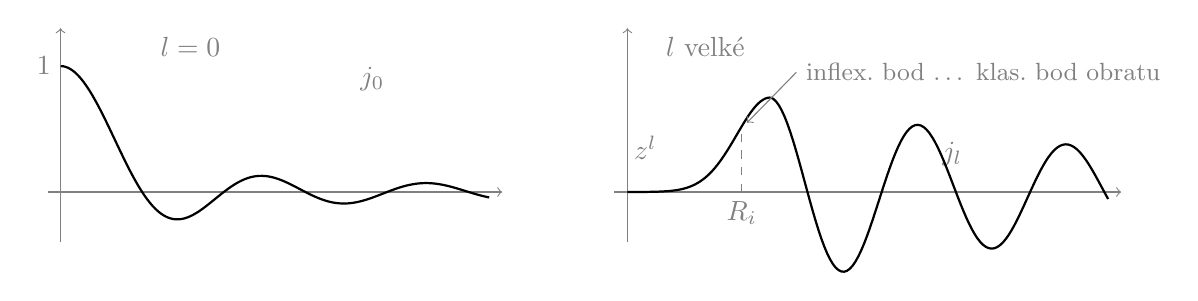
\begin{tikzpicture}[gray,x=0.33cm,y=1.6cm]
  % j0
  \draw[->] (-0.5,0) -- (17,0);
  \draw[->] (0,-0.4) -- (0,1.3);
  \node[left] at (0,1) {$1$};
  \node at (5,1.15) {$l = 0$};
  \node at (12,0.9) {$j_0$};
  \draw[thick,black,domain=0.01:16.5,samples=150] plot (\x,{sin(\x r)/\x});
  % jl, l velké
  \begin{scope}[xshift=7.2cm]
    \draw[->] (-0.5,0) -- (19,0);
    \draw[->] (0,-0.4) -- (0,1.3);
    \node at (3,1.15) {$l$ velké};
    \node at (12.5,0.3) {$j_l$};
    \node[left] at (1.5,0.35) {$z^l$};
    \draw[thick,black,domain=0:5.5,samples=60] plot (\x,{0.75*exp(-0.3*(5.5-\x)*(5.5-\x))});
    \draw[thick,black,domain=5.5:18.5,samples=120] plot (\x,{0.75*cos(deg(1.1*(\x-5.5)))*exp(-0.06*(\x-5.5))});
    \draw[dashed] (4.4,0) -- (4.4,0.52);
    \node[below] at (4.4,0) {$R_i$};
    \draw[<-] (4.6,0.55) -- (6.5,0.95) node[right] {\small inflex.\ bod \dots\ klas.\ bod obratu};
  \end{scope}
\end{tikzpicture}
\end{center}

+ \underline{Normování:} \quad $\displaystyle\int_0^\infty j_l(kr)\,j_l(k'r)\,r^2\dd r = \frac{\pi}{2k^2}\delta(k - k')$ \\
tj.\ \quad $\begin{cases}
  \braket{k'l'm'}{klm} = \displaystyle\int_0^\infty r^2\dd r\int\dd^2\vec n\,\psi_{k'l'm'}^*(r\vec n)\,\psi_{klm}(r\vec n) = \delta(k - k')\delta_{ll'}\delta_{mm'} \\[8pt]
  \displaystyle\sum_{lm}\int_0^\infty\dd k\,\psi_{klm}(\vec Q)\,\psi_{klm}^*(\vec Q\,') = \delta(\vec Q - \vec Q\,')
\end{cases}$ \\
\quad kde \quad $\vzorec{\psi_{klm}(r\vec n) = \sqrt{\frac{2}{\pi}}\,k\,j_l(kr)\,Y_{lm}(\vec n)}$

Energetická normalizace: \quad $\braket{E'l'm'}{Elm} = \delta(E - E')\delta_{ll'}\delta_{mm'}$
\[
  \psi_{Elm}(r\vec n) = \boxed{\frac1\hbar\sqrt{\frac{m}{k}}}\sqrt{\frac2\pi}\,k\,j_l(kr)\,Y_{lm}(\vec n) \qquad k = \sqrt{2mE}/\hbar
\]
\hspace*{3cm}\pozn{$\hookrightarrow\ \big[\frac{\dd E}{\dd k}\big]^{-1/2} = 1\big/\sqrt{\frac{\hbar^2k}{m}}$} \qquad \pozn{$\hookrightarrow E = \frac{\hbar^2k^2}{2m}$}

\underline{pozn:} Po částech konstantní potenciál ve 3D: \\
\quad napojování \quad $R_{kl}(r) = a\,j_l(\tilde kr) + b\,n_l(\tilde kr)$, \quad kde $\tilde k = \frac1\hbar\sqrt{2m(E - V)}$ \quad + spojité $R, R'$ \\
\quad + asymptotika \quad $h_l^{(\pm)}(z) \equiv j_l \pm in_l \xrightarrow{\ z\to\infty\ } \dfrac1z\underbrace{e^{\mp i(l+1)\frac{\pi}{2}}}_{(\mp i)^{l+1}}e^{\pm iz}$ \\
\quad\quad $\hookrightarrow$ \dots\ pro $\tilde k = i\varkappa$ \dots\ jen $h^{(+)}$ povolena v $+\infty$

\sout{$\delta$-chování v počátku:}

%----------------------------------------------------------------------
\strana{QM-C3-13}
\subsection*{5) \underline{Částice v radiálním poli} $\to$ ÚSKO \dots\ $H, L^2, L_z$}
\[
  \braket{\vec Q}{lmE} = \psi(x,y,z) = \psi(r,\theta,\varphi) = R_{El}(r)\,Y_{lm}(\theta,\varphi)
\]
\[
  H\psi = E\psi \ \Rightarrow\ -\boxed{\frac{\hbar^2}{2m}}\frac{1}{r^2}\Big[\pdv{r}r^2\pdv{r} - l(l+1)\Big]R_{kl}(r) + V(r)R_{kl} = ER_{kl}
  \quad\dots\ E = \frac{\hbar^2k^2}{2m}
\]
\[
  \to\quad R_{kl}''(r) + \frac2r R_{kl}' + \Big[k^2\underbrace{- \frac{l(l+1)}{r^2} - U(r)}_{(\star)}\Big]R_{kl}(r) = 0
\]
\[
  (\star) = -V_{\text{eff}}^{(l)}(r)\cdot\frac{2m}{\hbar^2} = -\frac{2m}{\hbar^2}\Big(V(r) + \frac{\overbrace{l(l+1)\hbar^2}^{L^2}}{2mr^2}\Big)
\]
kde: \quad $U(r) = \dfrac{2m}{\hbar^2}V(r)$ \quad nebo $\nearrow$
\[
  \text{nebo}\quad \vzorec{\chi''(r) + \Big[k^2 - \frac{l(l+1)}{r^2} - U(r)\Big]\chi(r) = 0}
\]

\underline{některé řešitelné případy:}
\subsubsection*{5a) \underline{Po částech konstantní potenciál:}}
zavedeme na každé části \quad $\varkappa^2 = k^2 - U$, \quad řešení známe:
\[
  R_{kl}(r) = a\,j_l(\varkappa r) + b\,n_l(\varkappa r)
\]
nebo \quad $\chi(r) = a\,r\,j_l(\varkappa r) + b\,r\,n_l(\varkappa r)$ \quad $\leftarrow$ hodí se hlavně pro $l = 0$, kde $j_l = \frac{\sin z}{z}$, $n_l = -\frac{\cos z}{z}$

+ \underline{okrajové podmínky:} \quad $\chi(r)\big|_{r=0} = 0$ \quad $\to$ \quad \underline{$b = 0$ na prvním úseku}

pro vázané stavy: na úsecích, kde $E < V$ \dots\ tj.\ $k^2 < U$ \dots\ $\varkappa$ ryze imag.\ $= i\lambda$ \\
\quad hodí se zavést: \quad $h_l^{(\pm)}(z) = j_l(z) \pm in_l(z) \xrightarrow{\ z\to\infty\ } (\mp i)^{l+1}\frac1z e^{\pm iz}$

\quad př: pro $h^{(+)}\approx\frac1z\big(\sin(kr - \frac l2\pi) - i\cos(kr - \frac l2\pi)\big) = \frac{-i}{z}e^{i(kr - \frac l2\pi)}$

\quad \dots\ \underline{na posledním úseku} \quad $R_{kl}(r) = a\,h_l^{(+)}(\varkappa r)$ + \sout{$b\,h_l^{(-)}(\varkappa r)$} \hfill {\color{gray}$b = 0$} \\
\hspace*{6.6cm} $\downarrow$ \hspace*{1.7cm} $\downarrow$ \\
\hspace*{6.3cm} $e^{-\lambda r}$ \hspace*{1.4cm} $e^{+\lambda r}$ \qquad $r\to\infty$

\underline{napojování:} spojité $R, R'$ nebo $\chi,\chi'$ \dots\ dá se dělat pomocí $(\ln\chi)'$, $(\ln R)'$ \\
\hspace*{5.5cm} \dots\ nezávisle na norm.

\subsubsection*{5b) \underline{Částice v Coulombickém poli} \quad $V(r) = \frac{\gamma}{r}$ \dots\ $\gamma < 0$ \dots\ přitažlivý}
\hfill\pozn{rozptyl. stavy později}

\underline{pozn:}
\begin{itemize}[nosep]
  \item důležitý případ $\to$ atom vodíku + ionty \\
        \hspace*{2.75cm} $\to$ muonium, protonium, pozitronium \dots \\
        \hspace*{2.75cm} $\to$ báze se využívá při výpočtech
  \item vyšší symetrie (dynamická) -- Runge-Lenzův vektor \\
        $\to$ \uv{náhodná} degenerace \\
        -- separabilní ve sférických, parabolických, eliptických souř.\ (což se někdy hodí)
  \item kvalitativní diskuse v termínech $V_{\text{eff}}^{(l)}(r)$
\end{itemize}

%----------------------------------------------------------------------
\strana{QM-C3-14}
\underline{Radiální (SR):} \quad \dots\ opět se dá řešit algebraicky pomocí posun.\ oper. \\
\hspace*{2.5cm} $\to$ zde \dots\ stručné shrnutí řešení dif.\ rovnice
\[
  \chi''(r) + \frac{2m}{\hbar^2}\Big[E \pm \frac{|\gamma|}{r} - \frac{\hbar^2 l(l+1)}{2mr^2}\Big]\chi(r) = 0
  \qquad\dots\ \begin{tabular}{l} $+|\gamma|$ \dots\ přitažlivý \\ $-|\gamma|$ \dots\ odpudivý\end{tabular}
\]
\hspace*{6cm}{\color{vetabarva}\dots\ diskutovat obrázkem}

přepis do bezrozm.: \quad $\rho = \beta r$ \dots\ $\beta$ \dots\ 1/délka \quad \dots\ $\chi(r) = u(\rho)$
\[
  \to\quad u'' + \underbrace{\boxed{\frac{2mE}{\hbar^2\beta^2}}}_{\text{bezrozm.}}u \pm \boxed{\frac{\gamma 2m}{\hbar^2\beta}}\cdot\frac{u}{\rho} - \frac{l(l+1)}{\rho^2}u = 0
\]
\quad $\hookrightarrow$ bezrozm.\ \dots\ standard $= \frac14$ \dots\ tj.\ $\beta = \sqrt{\dfrac{8m|E|}{\hbar^2}}$ \\
\quad\quad $\hookrightarrow$ \quad $\lambda = \dfrac{2m|\gamma|}{\beta\hbar^2} = \dfrac{|\gamma|}{\hbar}\sqrt{\dfrac{m}{2|E|}}$
\[
  \to\quad \vzorec{u'' + \Big[-\frac14 + \frac\lambda\rho - \frac{l(l+1)}{\rho^2}\Big]u = 0}
\]
\hspace*{3cm}\pozn{$\uparrow$ pro $E < 0$, jinak $(+)$} \quad \pozn{$\uparrow$ pro $\gamma < 0$, jinak $(-)$}

\underline{asymptotika}: \quad $\rho\to 0$ \dots\ stejně jako volná č.\ ($\frac\lambda\rho$ méně singul.\ než $\frac{l(l+1)}{\rho^2}$) \\
\hspace*{3cm} \dots\ tj.\ $u(\rho)\sim\rho^{l+1}$ \dots\ regulární řešení \\
$\rho\to\infty$ \quad \dots\ $u'' = \frac14u$ \quad $\to$ \quad $u(\rho) = e^{\pm\rho/2}$, \quad $\to$ přežije $\ominus$

\underline{položíme}: \quad $u(\rho) = \rho^{l+1}e^{-\rho/2}w(\rho)$:
\[
  \rho w'' + (2l + 2 - \rho)w' + \big[\lambda - (l+1)\big]w = 0
\]
\rule{\linewidth}{0.3pt}

\begin{minipage}[t]{0.55\textwidth}
\underline{ODBOČKA:} \dots\ široká třída ODR 2.\ ř.\ lze převést na (Formánek):

\underline{Gaussova rovnice:}
\[ z(1-z)\bar w'' + \big[c - (1+a+b)z\big]\bar w' - ab\,\bar w = 0 \]
definuje \kw{hypergeometrickou funkci}: \\
\quad $F(a,b,c,z)$ \dots\ lze řešit řadou
\end{minipage}
\vrule\hspace{6pt}
\begin{minipage}[t]{0.42\textwidth}
\underline{Degenerovaný případ:}
\[ \rho w'' + (c - \rho)w' - aw = 0 \]
\[ \to\quad F(a,c,\rho) = \lim_{b\to\infty}F\Big(a,b,c,\frac\rho b\Big) \]
\end{minipage}

\rule{\linewidth}{0.3pt}
\dots\ řešení řadou dá: \quad $w_1(\rho) = F(a,c,\rho) = 1 + \dfrac{1}{1!}\dfrac{a}{c}\rho + \dfrac{1}{2!}\dfrac{a(a+1)}{c(c+1)}\rho^2 + \dots$ \\
\hspace*{2.5cm} druhé řeš.: \quad $w_2(\rho) = \rho^{1-c}F(1+a-c,\,2-c,\,\rho)$ \dots\ singul.\ v poč.

\underline{náš problém:} \quad $c = 2(l+1)$, \quad $a = l + 1 - \lambda$

řada se pro $a = 0,-1,-2,\dots$ redukuje na polynom. \\
jinak se dá DK: \quad $F(a,c,\rho)\sim e^\rho$ \dots\ tj.\ $u = \rho^{l+1}we^{-\rho/2}\sim e^{+\rho/2}$ \ \pozor{špatné}

$\Rightarrow$ \kw{kvantovací podmínka}: \quad $a = l + 1 - \lambda = -\nu$ \quad \dots\ $\nu = 0,1,2,\dots$ \\
\hspace*{6.5cm} $\uparrow$ lze splnit jen pro $\gamma < 0$, jinak je tady $\oplus$
\[
  \hookrightarrow\ \text{tj.}\ \lambda^2 = \frac{\gamma^2}{\hbar^2}\frac{m}{2|E|}
  \ \to\ \vzorec{E_n = -\frac{m\gamma^2}{2\hbar^2n^2} = -\frac{\mathrm{Ry}}{n^2}}
  \quad\nwarrow\ \text{vodík } \gamma = -\frac{e^2}{4\pi\varepsilon_0}\ (\mathrm{SI})
\]
\hspace*{11cm} $\to 1\,\mathrm{Ry} = 13.6\,\mathrm{eV} = \frac12\,\mathrm{Ha}$

\quad kde \quad $n = \nu + l + 1$ \quad \dots\ \kw{hlavní kvantové číslo} \\
\quad\quad \dots\ význam $\nu$ \dots\ řád polynomu $=$ počet nul $R_{nl}(r)$ \quad {\color{vetabarva}radiální kvantové číslo}

%----------------------------------------------------------------------
\strana{QM-C3-15}
\underline{systematizace hladin:} \quad $n = l+1, l+2,\dots$ \\
\quad nebo \quad $n = 1,2,3,\dots$; \quad $l = 0,1,\dots,n-1$; \quad $m = -l,-l+1,\dots,l$

\begin{minipage}{0.75\textwidth}
stupeň degenerace pro dané $E_n$ \dots\ $\vzorec{N = \sum_{l=0}^{n-1}(2l+1) = n^2}$ \\
$\to$ \uv{Náhodná degenerace} \\
\quad \dots\ ve skutečném H \dots\ další st.\ volnosti: \quad
$\begin{aligned}[t] &\text{spin } e^- \dots\ 2n^2 \\ &\text{spin } p^+ \dots\ 4n^2\end{aligned}$
\end{minipage}
\begin{minipage}{0.23\textwidth}
$\Bigg\}$ \small sejmutí degenerace po započt.\ korekcí \dots\ Dirac, pole
\end{minipage}

\underline{typické rozměry atomu:} \quad
$\rho = \beta r = \dfrac{\sqrt{8m|E_n|}}{\hbar}r = \dfrac{\sqrt{4m\frac{m\gamma^2}{\hbar^2n^2}}}{\hbar} = \dfrac{2m|\gamma|}{\hbar^2n}\cdot r$
\[
  \rho = \frac{2r}{na} \quad\dots\ \text{kde}\quad
  \boxed{\begin{aligned} a &= \Big[\frac{m|\gamma|}{\hbar^2}\Big]^{-1} \doteq 0.53\,\text{Å} \\ &\text{\kw{Bohrův poloměr}}\end{aligned}}
\]

\underline{Vlnové funkce:}
\[
  R_{nl}(r) = N_{nl}\underbrace{\Big(\frac{2r}{na}\Big)^l}_{\rho}\underbrace{F\big(-\nu,\,2(l+1),\,\rho\big)}_{\hookrightarrow\ \text{(zobecněný) Laguerův polynom}}e^{-\rho/2}
\]
def: \quad $L_n^\alpha(x) \equiv \dbinom{n+\alpha}{n}F(-n,\alpha+1,x)$
\[
  \to\quad \vzorec{R_{nl}(r) = \frac2n\sqrt{\frac{(n-l-1)!}{(n+l)!}}\;a^{-\frac32}\Big(\frac{2r}{na}\Big)^lL_\nu^{2l+1}\Big(\frac{2r}{na}\Big)e^{-\frac{r}{na}}}
  \qquad \nu = n - l - 1
\]

\underline{více o Laguer.\ polynomech}
\begin{itemize}
  \item altern.\ def: \quad $L_n^\alpha(x) = \displaystyle\sum_{m=0}^{n}(-1)^m\binom{n+\alpha}{n-m}\frac{x^m}{m!} = \frac{1}{n!}e^xx^{-\alpha}\frac{\dd^n}{\dd x^n}\big(e^{-x}x^{n+\alpha}\big)$
  \item ortogonální systém vůči míře $e^{-z}z^\alpha$ \\
  tj.\ \quad $\displaystyle\int_0^\infty L_n^\alpha(x)\,L_{n'}^\alpha(x)\,x^\alpha e^{-x}\,\dd x = \delta_{nn'}\frac{\Gamma(\alpha+n+1)}{n!}$
\end{itemize}

\underline{Pár prvních stavů:}
\begin{align*}
  R_{10}(r) &= 2\sqrt{\tfrac{1}{a^3}}\;e^{-r/a} \qquad\leftarrow\ \text{základní} \\
  R_{20}(r) &= \sqrt{\tfrac{1}{2a^3}}\Big[1 - \frac{r}{2a}\Big]e^{-r/2a} \\
  R_{21}(r) &= \tfrac12\sqrt{\tfrac{1}{6a^3}}\;\frac ra\,e^{-r/2a} \\
  &\ \ \vdots
\end{align*}

%----------------------------------------------------------------------
\strana{QM-C3-16}
\subsubsection*{5c) \underline{Izotropní 3D LHO}}
\[
  V(r) = \tfrac12 m\omega^2r^2 \qquad \big(= \tfrac12m(\omega^2x^2 + \omega^2y^2 + \omega^2z^2)\big)
\]
$\to$ \quad $\psi_{Elm}(x) = R_{nl}(r)\,Y_{lm}(\theta,\varphi)$ \quad \dots\ $\chi = rR$
\[
  \to\quad \chi''(r) + \frac{2m}{\hbar^2}\Big(E - \frac12m\omega^2r^2 - \frac{\hbar^2l(l+1)}{2mr^2}\Big)\chi = 0
\]
\quad \dots\ škálování \quad $x_0 = \sqrt{\dfrac{\hbar}{m\omega}}$ \quad \dots\ $r = \rho x_0$, \quad $\chi(r) = u(\rho)$
\[
  \to\quad u'' + \Big(\frac{2E}{\hbar\omega} - \rho^2 - \frac{l(l+1)}{\rho^2}\Big)u = 0
  \qquad\dots\ \lambda = \frac{2E}{\hbar\omega}\ \dots\ \text{bezrozm.\ energie}
\]
\quad \dots\ asymptotika \quad $\to$ \quad $u(\rho) = \rho^{l+1}e^{-\frac12\rho^2}w(\rho)$
\[
  \to\quad w''(\rho) + \frac2\rho\big((l+1) - \rho^2\big)w'(\rho) + (\lambda - 2l - 3)\,w(\rho) = 0
\]
\quad subst: \quad $z = \rho^2$ \quad \dots\ $w(\rho) = v(z)$
\[
  \to\quad z\,v'' + \big(\underbrace{l + \tfrac32}_{c} - z\big)v' + \big(\underbrace{\tfrac\lambda4 - \tfrac l2 - \tfrac34}_{-a}\big)v = 0
\]
\quad \dots\ opět rovnice pro degener.\ hypgeom.\ fci. \\
\quad\quad $\to$ řešení \dots\ Laguerovy polynomy \quad $v(z) = F(a,c,z)$

kvantovací podmínka: \quad $\frac34 + \frac l2 - \frac\lambda4 = a = -\nu$
\[
  \Rightarrow\quad \vzorec{E = 4\cdot\frac{\hbar\omega}{2}\Big(\nu + \frac l2 + \frac34\Big) = \hbar\omega\Big(\underbrace{2\nu + l}_{\Lambda} + \frac32\Big)}
  \qquad \nu = 0,1,\dots\quad l = 0,1,\dots
\]
\hspace*{7cm} $\Lambda$ \dots\ hlavní kvantové číslo

pro fixní $\Lambda$: \dots\ sudé: $l = 0,2,\dots,\Lambda$ \quad \dots\ $N_{\deg} = \sum_{l=0,2}^{\Lambda}(2l+1) = \frac12(\Lambda+1)(\Lambda+2)$ \quad \pozn{$= \frac12(\frac\Lambda2+1)(2\Lambda+2)$} \\
\hspace*{2.75cm} lichá: $l = 1,3,\dots,\Lambda$ \quad \dots\ $N_{\deg} = \sum_{l=1,3}^{\Lambda}(2l+1) = \frac12(\Lambda+1)(\Lambda+2)$ \quad \pozn{$= \frac12(\frac{\Lambda+1}{2})(2\Lambda+4)$}

\subsection*{6) \underline{Separabilní systém}}
\dots\ na Hilb.\ prostoru \quad $\mathcal{H} = \mathcal{H}^{(1)}\otimes\mathcal{H}^{(2)}$ \quad \dots\ $H = H_1 + H_2$ \\
\hspace*{4.5cm} $\hookrightarrow$ ÚSKO \dots\ $(H_1,A)$, \ $(H_2,B)$

$\Rightarrow$ $H_1, A, H_2, B$ \dots\ ÚSKO na $\mathcal{H}$ \\
\quad navíc \quad $\ket{\psi} = \ket{\psi^{(1)}}\otimes\ket{\psi^{(2)}} = \ket{E_1\alpha}\otimes\ket{E_2\beta}$
\[
  \text{a}\quad H\ket{\psi} = \big(H_1\ket{E_1\alpha}\big)\otimes\ket{E_2\beta} + \ket{E_1\alpha}\otimes\big(H_2\ket{E_2\beta}\big) = \vzorec{(E_1 + E_2)\ket{\psi}}
\]

\begin{priklad}[PŘ: Izotropní LHO]
\[
  E = E_x + E_y + E_z = \hbar\omega\Big(\frac32 + \underbrace{n_x + n_y + n_z}_{\Lambda}\Big)
\]
$\psi(x,y,z) = \psi_{n_x}(x)\,\psi_{n_y}(y)\,\psi_{n_z}(z)$

stupeň degenerace?
\begin{center}
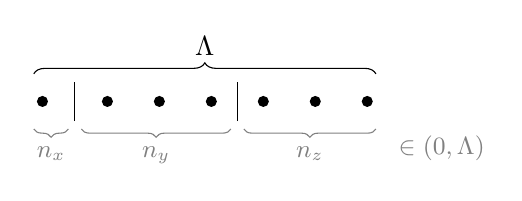
\begin{tikzpicture}[x=0.55cm]
  \foreach \x in {0,1.5,2.7,3.9,5.1,6.3,7.5} \fill (\x,0) circle (2pt);
  \draw (0.75,-0.25) -- (0.75,0.25);
  \draw (4.5,-0.25) -- (4.5,0.25);
  \draw[decorate,decoration={brace,amplitude=4pt}] (-0.2,0.35) -- (7.7,0.35) node[midway,above=3pt] {$\Lambda$};
  \draw[gray,decorate,decoration={brace,mirror,amplitude=3pt}] (-0.2,-0.35) -- (0.6,-0.35) node[midway,below=3pt] {\small $n_x$};
  \draw[gray,decorate,decoration={brace,mirror,amplitude=3pt}] (0.9,-0.35) -- (4.35,-0.35) node[midway,below=3pt] {\small $n_y$};
  \draw[gray,decorate,decoration={brace,mirror,amplitude=3pt}] (4.65,-0.35) -- (7.7,-0.35) node[midway,below=3pt] {\small $n_z$};
  \node[gray,right] at (8,-0.6) {\small $\in(0,\Lambda)$};
\end{tikzpicture}
\end{center}
\dots\ volím 2 přihrádky z $\Lambda + 1$ \dots\ kombinace s opakováním
\[
  N_{\deg} = \binom{\Lambda+1}{2} + \Lambda + 1 = \frac12(\Lambda+1)(\Lambda+2)
\]
\end{priklad}

%----------------------------------------------------------------------
\strana{QM-C3-17}
\begin{priklad}[Jiný příklad: Dvě částice interagující prostřednictvím $V(Q^{(1)} - Q^{(2)})$]
\underline{v klasické mechanice:} \quad
$L(\vec Q^{(1)},\vec Q^{(2)},\dot{\vec Q}^{(1)},\dot{\vec Q}^{(2)}) = \frac12M^{(1)}\dot{\vec Q}^{(1)2} + \frac12M^{(2)}\dot{\vec Q}^{(2)2} + V$

nové proměnné:
\[
  \begin{aligned}
    \vec X &= \frac{M^{(1)}\vec Q^{(1)} + M^{(2)}\vec Q^{(2)}}{M^{(1)} + M^{(2)}} &&\dots\ \text{CMS} \\
    \vec x &= \vec Q^{(1)} - \vec Q^{(2)} &&\dots\ \text{relat.\ poloha}
  \end{aligned}
  \quad\Rightarrow\quad
  \begin{aligned}
    \vec P &= \pdv{L}{\dot X} = \vec p^{(1)} + \vec p^{(2)} \\
    \vec\pi &= \pdv{L}{\dot x} = \frac{M^{(2)}\vec p^{(1)} - M^{(1)}\vec p^{(2)}}{M^{(1)} + M^{(2)}}
  \end{aligned}
\]
+ dá s DK: \quad
$H = \underbrace{\dfrac{\vec P^2}{2M}}_{\text{CMS}} + \boxed{\underbrace{\dfrac{\vec\pi^2}{2\mu} + V(\vec x)}_{\text{rel}}}$ \quad kde \quad $\vzorec{\mu = \frac{M_1M_2}{M_1 + M_2}}$

\underline{v kvantové mechanice:}
\begin{align*}
  H &= -\frac{\hbar^2}{2M^{(1)}}\Delta^{(1)} - \frac{\hbar^2}{2M^{(2)}}\Delta^{(2)} + V(Q^{(1)} - Q^{(2)}) \\
  &= -\frac{\hbar^2}{2M}\Delta_{\text{CMS}} - \frac{\hbar^2}{2\mu}\Delta_{\text{rel}} + V(\vec x) = H_{0\,\text{CMS}} + H_{\text{rel}}
\end{align*}
\rule{\linewidth}{0.3pt}
\underline{DK:}
\begin{align*}
  \pdv{Q^{(1)}} &= \pdv{X}{Q_1}\nabla_X + \pdv{x}{Q_1}\nabla_x = \frac{M_1}{M}\nabla_X + \nabla_x
  &&\to\ \Delta_Q^{(1)} = \frac{M_1^2}{M^2}\Delta_X + \Delta_x + \frac{2M_1}{M}\nabla_X\cdot\nabla_x \\
  \nabla_{Q^{(2)}} &= \pdv{X}{Q_2}\nabla_X + \pdv{x}{Q_2}\cdot\nabla_x = \frac{M_2}{M}\nabla_X - \nabla_x
  &&\to\ \Delta_Q^{(2)} = \frac{M_2^2}{M^2}\Delta_X + \Delta_x - \frac{2M_2}{M}\nabla_X\cdot\nabla_x
\end{align*}
\[
  \frac{1}{M_1}\Delta^{(1)} + \frac{1}{M_2}\Delta^{(2)} = \frac1M\Delta_X + \frac{M_1 + M_2}{M_1M_2}\Delta_x
\]
\rule{\linewidth}{0.3pt}

\underline{Důsledek:} \quad $\mathcal{H} = \mathcal{H}^{(1)}\otimes\mathcal{H}^{(2)} = \mathcal{H}^{(\text{CMS})}\otimes\mathcal{H}^{(\text{rel})}$ \\
\hspace*{2cm} $H = H_{0\,\text{CMS}} + H_{\text{rel}}$ \hfill \pozn{pro $V(\vec x) = V(|\vec x|)$ \dots\ sfér.\ symetrie} \\
$\to$ stacionární stavy \quad $\ket{\psi} = \ket{\vec P_{\text{CMS}}}\otimes\ket{Elm}$ \\
\quad \dots\ tj.\ např.\ atom vodíku v souř.\ reprezentaci:
\[
  \psi(\vec X,\underbrace{\vec x}_{=r\vec n}) = \frac{1}{\sqrt{(2\pi\hbar)^3}}\,e^{\frac{i}{\hbar}\vec P_{\text{CMS}}\cdot\vec X}\cdot R_{nl}(r)\,Y_{lm}(\vec n)
\]
$\to$ jediné, čím se pozná, že 2-částicový syst.\ \dots\ $M\to\mu = \dfrac{M_1M_2}{M_1 + M_2}$

\dots\ stejné jako $H = pe$ je $e^+e^-$ (pozitronium), $p^+\mu^-$, $p^+\bar p$ (protonium), $de^-$ (deuterium) \\
\hspace*{2cm} $\to$ liší se jen $\mu$ \quad \dots\ př.\ \dots\ $m_e$ od $\mu$ pro H se liší o méně než $1\,$\textperthousand
\end{priklad}

